\chapter{英文法に関するいくつかの重要な概念、用語、そして考え方}\label{ch:1}

\begin{tblsframedsymbol}{学習目標}{bulb}
  \begin{itemize}[noitemsep, leftmargin=*]
      \item 言語学的な定義において、必要十分条件がなぜ機能しないのかを理解する
      \item 文法用語の日常的な意味と専門的な意味を区別する
      \item 反例を探すなど、批判的思考（クリティカル・シンキング）の戦略を応用する
      \item 英語の基本的な語彙範疇（名詞、動詞、形容詞、限定詞）を識別し始める
      \item 文脈によって、単語がどのように異なる範疇に属し得るかを認識する
      \item 語彙範疇が、規則ベースではなくプロトタイプに基づく概念であることを理解する
      \item 境界事例（グレーゾーン）があっても、語彙範疇を識別するための体系的な基準を適用する
      \item 一見単純に見える文法概念の根底にある複雑さを理解する
  \end{itemize}
  \end{tblsframedsymbol}

\section{はじめに}\label{sec:intro1}

英文法を教えるという考えに緊張を感じるとしても、あなたは一人ではありません。英語教師を志す多くの人が文法に苦手意識を持ち、副詞と形容詞の違いに自信が持てなかったり、自分が教えようとしている言語の複雑さについて十分な知識がないのではないかと不安に思ったりしています。しかし、ここで秘密をお教えしましょう。文法を理解するというのは、堅苦しいルールのセットを暗記することではありません。もちろん暗記すべきこともありますが、言語についての新しい考え方を身につけない限り、それはあまり役に立ちません。その新しい考え方こそが、あなたが英語を理解し、ひいては将来の生徒たちが英語を理解するのを助けるものなのです。

この章は、皆さんがこの新しい考え方にスムーズに入れるように設計されています。\term{接語（clitic）}、\term{直示（deixis）}、\term{能格（ergative）}といった全く馴染みのない用語をいきなり浴びせたり、複雑な規則を並べ立てたりするつもりはありません。その代わりに、言語に関するいくつかの基本的な前提に疑問を投げかけ、私たちが理解していると思っている物事をどのように定義しているのかを探求することから始めます。

いくつかの基本的な概念から始めて、徐々により具体的な文法のアイデアへと構築していきます。その過程で、言語を教えようとするすべての人にとって不可欠な批判的思考の戦略を発展させていきます。反例を探し、異なる視点を考慮し、用語の日常的な使い方と専門的な使い方の違いを認識することを学びます。

英語\enquote{について}多くを知ることに何の価値があるのかと懐疑的に思っているなら、それもまたあなただけではありません。しかし、教師の言語に対する意識（Teacher Language Awareness: TLA）に関する研究は、言語がシステムとしてどのように機能するかを理解している教師の方が、学習者のエラーを診断し、困難を予測し、その場で説明を適応させる能力が高いことを示唆しています \autocite{Andrews2007}。Stevickが述べているように、教師は言語の道筋と障害物を知る必要があります。\enquote{自分自身がその中を行ったり来たりするためだけでなく、新参者（学習者）にとってそれがどのように見えるかを見るため}です（\citeyear{Stevick1980}: 251, cited in \citealt{Andrews2007}: 7）。誤解しないでください。この本は生徒に言語学を教えられるようになるためのものではありません。教師であるあなたが、生徒の問題を予測し、それに対応し、流暢な話者が無意識に行っていることを言葉で説明するために知っておくべきことについての本です。

しかし、何かが知識として数えられるためには、それが真実でなければなりません。そして、言語に関する知識として通用しているものの多くは、このテストに合格しません。\enquote{名詞は人、場所、物である}\enquote{動詞は動作を表す言葉である}——これらは言語についての信念であって、知識ではありません。\textcite{Bartels2009} は、言語に関する学術的な知識が自動的に教室での実践に移行するわけではないと警告しています。私に言わせれば、それは部分的にはそれが真の知識の基準を満たしていないからです。言語に関する真の知識は、教師がそれを教室の要求と結びつけたときに有用になります。そして、この本にはその結びつけを助けるための多くの練習問題が含まれています。

今の時点で自分の文法知識に自信がなくても心配しないでください。この章が終わる頃には、言語について考えるための基本的なツールキットを手に入れ、より自信を持って文法に取り組むことができるようになるでしょう。では、最初は単純に見えるかもしれませんが、より深く考えることを要求する質問から始めましょう。\enquote{スープをスープたらしめているものは何でしょうか？}

答えるまでは、馬鹿げていて、無関係で、些細なほど簡単な質問に思えるかもしれません。お茶とスープ、ソースとスープ、お粥とスープ、シチューとスープ、ジュースとスープの違いは何でしょうか？ガスパチョ、サルモレホ、キュウリスープなど、冷たいスープがあることも忘れないでください。\footnote{出典: BBC Scotland (\url{https://youtu.be/Y1HVTNxwt7w})}

これはスープに限ったことではありません。ほとんどの物事は、例や反例を見始めると、明確に定義するのが非常に難しいことがわかります。問題は、私たちが\textbf{必要十分条件}を選び出すことで物事を定義しようとすることにあります。

\subsection{必要十分条件}\label{sec:conditions}

\is{definition!necessary and sufficient conditions|(}\is{necessary and sufficient conditions|(}哲学的および科学的な分野の双方において、\term{必要十分条件}（necessary and sufficient conditions）という概念が見られます。必要条件とは、承認されるために存在しなければならない条件であり、十分条件とは、存在すれば承認が保証される条件のことです。言い換えれば、ある単語が名詞として分類されるための必要十分条件が条件Aであると言うとき、それは\enquote{その単語は特徴Aを持っていなければ名詞にはなれず（必要条件）}、\enquote{特徴Aが存在すればその単語は間違いなく名詞である（十分条件）}ということを意味します。

これについての明確で分かりやすい例は、数学における偶数の概念です。整数を2で割った結果が別の整数になる場合、その整数は偶数です。これは整数が偶数であるための必要十分条件です。このように2で割り切れない偶数は存在せず（必要条件）、そのような数は常に偶数です（十分条件）。\footnote{偶数と奇数の違いのように一見決定的に思えることでも、私たちが考えているほど明確ではないかもしれません \autocite{Heubner2018}。}\is{necessary and sufficient conditions|)}\is{definition!necessary and sufficient conditions|)}

このように、哲学的な抽象概念から数学的な確実性に至るまで、必要十分条件はしばしば私たちの概念理解の枠組みとなっています。

\subsection{（言語学的）定義の難しさ}\label{sec:definitions}

\is{definition!linguistic!challenge|(}しかし、言語やその構成要素になると、必要十分条件を用いた定義は機能しなくなる傾向があります。仮に、\is{noun, noun phrase (NP)|(}名詞（noun）を\enquote{人、場所、または物を表す言葉}と定義し、\is{verb, verb phrase (VP)|(}動詞（verb）を\enquote{動作を表す言葉}と定義したとしましょう。\mention{action}（行動・動作）という単語以上に動作を表す言葉が他にあるか、少し考えてみてください。そして、\mention{action} が動詞なのか名詞なのかを考えてみてください（ヒント：辞書\footnote{\url{https://www.ldoceonline.com/}}で確認してみましょう）。

はっきりさせておくと、\mention{action} は通常名詞ですが、動詞でもあります（例：\textit{We need to \emph{action} these tasks before the end of the day.} \enquote{今日中にこれらのタスクを実行する必要がある}）。あるいは、より一般的な名詞としての \mention{action} と、比較的珍しい動詞としての \mention{action} の2つが存在すると言った方が良いかもしれません。

しかし、\mention{action} だけではありません。\mention{violation}（違反）の定義\footnote{\url{https://www.ldoceonline.com/dictionary/violation}}を考えてみてください。これは名詞であり、かつ動作です。同じことが、\mention{blow} から \mention{cue}、\mention{signal} から \mention{sin} に至るまで、多くの名詞に当てはまります。これらは\enquote{the action of...（～の動作）}というフレーズを使って定義されており、\enquote{名詞は人、場所、物であり、動詞は動作を表す言葉である}という非常に一般的な考え方を完全に打ち砕いています。\is{noun, noun phrase (NP)!denotation}名詞も動作を表す言葉になり得るのです。\is{verb, verb phrase (VP)|)}\is{noun, noun phrase (NP)|)}

私たちは言語を理解するために単語を定義しますが、単語を定義するためには言語を理解する必要があるのです。

\begin{tblsframed}{思考の罠}
    \is{thinking trap!confirmation bias|(}テーブルの上に4枚のカードがあります。それぞれのカードは片面に数字が、もう片面に色が印刷されています。見えている面には\enquote{3}\enquote{8}\enquote{青}\enquote{赤}とあります。\enquote{もしカードの片面が偶数なら、もう片面は青である}というルールを確認するためには、どのカードを裏返す必要があるでしょうか？
    \begin{center}
        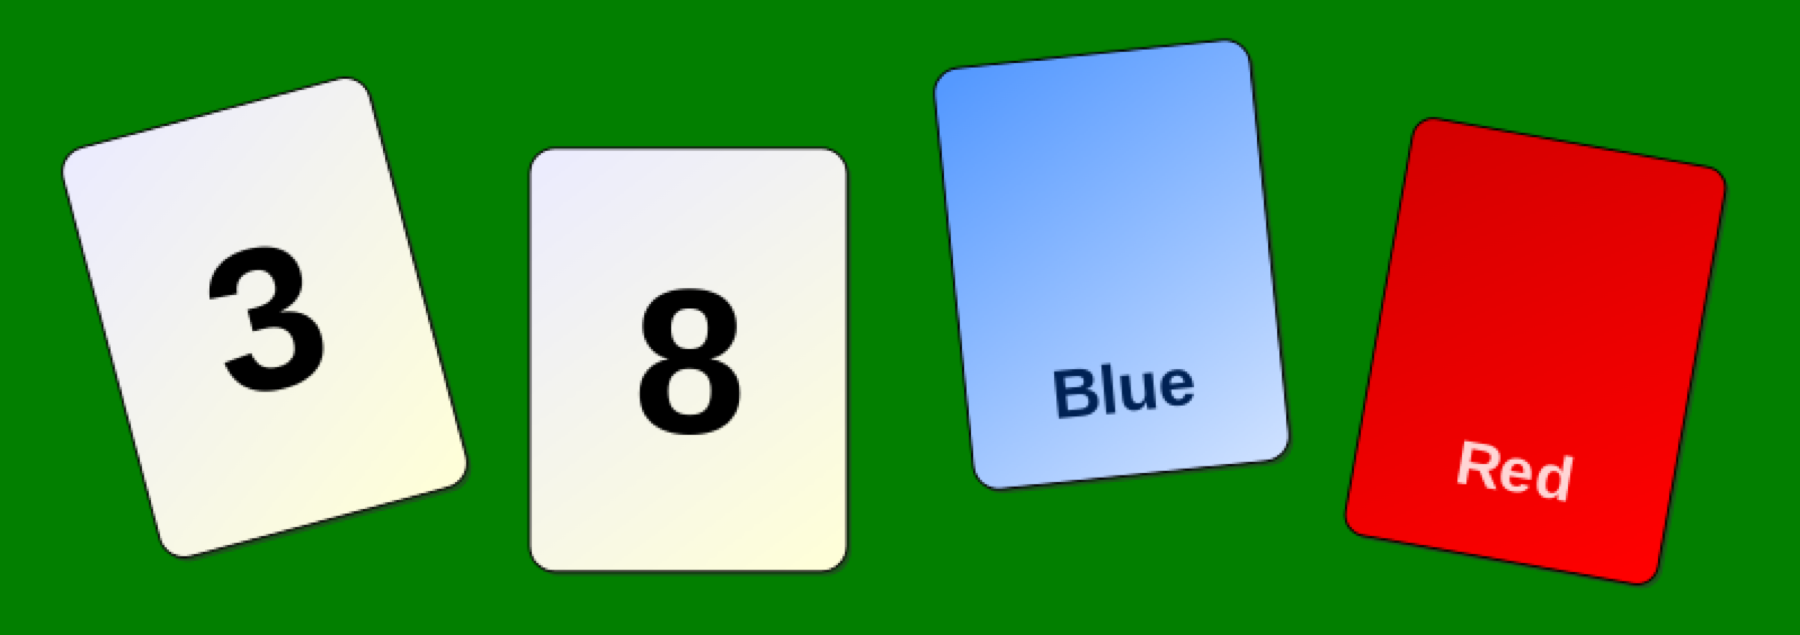
\includegraphics[width=0.5\textwidth]{figures/wason.png}
        \tiny \captionof{figure}{Image by User:Life of Riley and User:Domdomegg, CC BY-SA 4.0 via Wikimedia Commons.}

        \tiny License: \url{https://creativecommons.org/licenses/by-sa/4.0}
    \end{center}
    \indent 多くの人は\enquote{8}と\enquote{青}と答えるでしょう。確かに、\enquote{8}は確認する必要があります。裏側が青でなければ、ルールは破られていることになります。一方で、青いカードを裏返してもルールのテストにはなりません。ルールは偶数について述べているだけで、奇数については何も述べていないからです。これが、ほとんど誰も\enquote{3}のカードを確認しない理由でしょう。つまり、青いカードの裏が偶数であろうと奇数であろうと、ルールには影響しません。鍵を握るのは\enquote{赤}のカードです。これを裏返して偶数が出てきたら、ルールは破られていることになります。

    \is{counter-example}私たちの目標は、ルールを肯定するだけでなく、ルールが機能しない状況、つまり反例（counter-examples）を探すことでもあります。これは言語学的な概念の定義においても同様に重要です。メンバーでないものを含めたり、メンバーであるものを除外したりする定義は、良い定義とは言えません。\enquote{動作を表す言葉}を動詞の定義として評価する場合、肯定的な証拠と否定的な証拠の両方を考慮する必要があります。たとえば、\mention{run} という単語が\enquote{動作を表す言葉}であるか（そうです）、そして動詞であるか（そうです）を確認できます。一方で、\mention{action} や \mention{I went for a run} という文の \mention{run} のように、\enquote{動作を表す言葉}と考えられているのに動詞ではない単語などの否定的な証拠も探す必要があります。また、\mention{exist} や \mention{sense} のような必ずしも\enquote{動作を表す言葉}と認識されない単語も動詞になり得ます。\is{thinking trap!confirmation bias|)}

\end{tblsframed}

\is{noun, noun phrase (NP)!vs verb|(}\is{verb, verb phrase (VP)!vs noun|(}しかし、ここで何かを救済できるかもしれません。物理的な対象を表す言葉で、動詞であるものを思いつきますか？少し考えてみてください。

\bigskip

\is{noun, noun phrase (NP)!denotation}名詞と動詞はどちらも動作を表すことができると言って差し支えありませんが、\is{verb, verb phrase (VP)!denotation}動詞は決して物理的な対象や、人、場所を表すことはありません。そのためには名詞が必要です。このことは、私たちを次のような結論に導きます。
\ea
    \ea \enquote{人、場所、物は名詞によってのみ表される}というのは真ですが、
    \ex \enquote{名詞は人、場所、物のみを表す}というのは偽です。
    \z
\z
これは微妙な違いですが、重要な違いです。名詞はより多様なものを表すことができる一方で、動詞はより限定的であり、名詞と動詞が表すことができるものの集合は重なり合っています。\is{noun, noun phrase (NP)!vs verb|)}\is{verb, verb phrase (VP)!vs noun|)}

これまで、名詞と動詞を定義する際の3つの問題を特定しました。形容詞や他の語彙範疇に関しても同様の点が当てはまりますが、ここで一旦状況を整理しておきましょう。
\begin{enumerate}[noitemsep]
    \item 必要十分条件を用いた単純な定義は、属さないものを含めてしまい（グレービーソースはストックから作られますがスープではありません）、属するものを除外してしまいます（ガスパチョは冷たくして提供されますがスープです）。
    \item 念頭にある例に合うように定義を作るだけではいけません。意識的に\is{counter-example}反例（counter-examples）を考える必要があります。
    \item 自分の考えを正確に表現するために、言い換える必要がある場合があります。
\end{enumerate}\is{definition!linguistic!challenge|)}

語学教師として、私たちは\term{noun}（名詞）や\term{verb}（動詞）といったカテゴリー（範疇）をよく使います。しかし、単語を分類することはツールであり、最終目標ではありません。分類の目的は、世界について、あるいは今回の場合であれば言語について、一般的な記述ができるようにすることです。

これがなぜ重要なのかというと、間違ったカテゴリーは、必要以上に多くの\enquote{規則}と\enquote{例外}を生み出してしまうからです。正しいカテゴリーを持つということは、より少ない言葉でより多くのことを説明できるということであり、これによりあなたとあなたの生徒たちの両方にとって負担が軽減されます。

\bigskip

\begin{tblsframedsymbol}{質問}{test}
\begin{enumerate}[noitemsep, leftmargin=*]
    \item このコースの主な目標は何ですか？
    \item 英語の名詞は人、場所、物の名前であるという考えの何が間違っているのでしょうか？
    \item 次のうち、英語の動詞の必要十分な定義となっている文はどれですか： A) 動詞は動作を表す。 B) 動作は動詞によって表される。 C) どちらでもない。\is{necessary and sufficient conditions}
    \item スープのビデオは、単語のカテゴリーを定義することとどのように関連していますか？
    \item 私たちが避けるべき\enquote{思考の罠}とは何ですか？
\end{enumerate}
\end{tblsframedsymbol}

\begin{tblsfilled}{解答}
\begin{enumerate}[noitemsep, leftmargin=*]
    \item 言語分析の能力を高め、生徒が英語をどのように話すかを決定する際に使えるツールを提供できるようにすることです。
    \item 英語において、名詞は動作や特徴など、これよりもはるかに幅広い概念を表すからです。
    \item C) が正解です。動詞というカテゴリーは、その指示対象に基づいて確実に定義することはできません。
    \item 一般的に、カテゴリーには必要十分な特性がないことを説明しています。
    \item 自分の仮説を裏付ける肯定的な証拠だけを探し、仮説を覆すかもしれない証拠を探し損ねてしまうことです（確証バイアス）。
\end{enumerate}
\end{tblsfilled}

\subsection{\mention{phrase}（句）とはどういう意味か？}\label{sec:phrases}

\is{phrase!technical vs everyday meaning|(}名詞と動詞で見たように、言語に関する私たちの最も基本的な前提のいくつかが、私たちをつまずかせることがあります。たとえば、\mention{phrase} という単語を取り上げてみましょう。皆さんはおそらくその意味を知っていると思っているでしょう（結局のところ、私たちは毎日フレーズを使っています）。日常言語において、フレーズ（句）とは、\mention{on the table} や \mention{be going to} のように、アイデアを表現するために一緒になる単語のグループに過ぎません。そして、それは \mention{phrase} の完璧に適切な意味です。それは最も一般的なものであり、ほとんどの人がその単語から連想するものです。

しかし、専門的な意味も存在し、本書全体を通して私が使用するのはそちらの意味です。\is{phrase!as a headed structure|(}英文法における \term{phrase}（句）は、2つの重要な特性を持つ特定のタイプの構造です。
\begin{enumerate}[noitemsep]
    \item 句全体の基本的な特性を決定する中心的な単語である \is{head (function)!in phrase structure}\textsc{head}（主要部）を持っている
    \item 主要部の意味を修飾したり完成させたりする任意の単語や他の句である \is{dependent (Dep)}\term{従属部（dependents）}を持つことができる
\end{enumerate}\is{phrase!as a headed structure|)}
これは、\enquote{一緒になる言葉}という日常的な概念とは大きく異なります。たとえば、\mention{coffee and tea} は日常会話では完璧に良いフレーズのように思えるかもしれませんが、専門的には単一の句ではありません。それは \mention{and} で結ばれた2つの名詞句（\mention{coffee} と \mention{tea}）の等位接続です（等位接続についてはセクション~\ref{sec:coordination}を参照）。これらの単語のどれも、表現全体の主要部ではありません。

日常的な意味でのフレーズであって、専門的な意味での句ではないものの例には、以下のものが含まれます。

\setlength{\columnsep}{0pt}
\begin{multicols}{2}
\ea
    \ea \label{ex:missing_dependents} can't help but
    \ex let alone
    \ex \label{ex:missing_dep_context} {\ob}want to{\cb} try again
    \ex {\ob}pick up{\cb} the pencil
    \ex good or bad\label{ex:missing_head}
    \ex  salt and pepper
\z
\z
\end{multicols}
(\ref{ex:missing_dependents} と b) の例は、必要な従属部が欠けています。\mention{this isn't working, let alone} とは言えません。(\ref{ex:missing_dep_context} と d) の例は、完全な句を形成できる括弧で囲まれた部分（\mention{want to try again}、\mention{pick up the pencil}）を示していますが、完全な文脈から人工的に抽出されたものです。

(\ref{ex:missing_head} と f) の等位接続の例は、全く異なる問題を提示しています。私たちが議論してきた主要部を持つ構造とは異なり、等位接続は単一の主要部なしに同等のステータスの要素を結びつけます。私たちが \mention{salt and pepper} と言うとき、どちらの名詞も他方を認可（ライセンス）するわけではありません。それらは単に同等なのです。これにより、等位接続は主要部を必要とする専門的な意味での句とは根本的に異なるものになります。

今のところ、句とは何かについて深く考えすぎる必要はありません。ただ、私が \mention{phrase}（句）という言葉を、馴染みがあるように見えて実は微妙に異なる方法で使用するという事実に注意を促したいだけです。\is{phrase!technical vs everyday meaning|)}

\mention{phrase} の専門的な意味と日常的な意味の間のこの区別は、それほど珍しいことではありません。学者はしばしば一般的な言葉を採用しますが、それに専門的な意味を与えます。これは、日常的な意味が間違っているとか、専門的な意味が間違っているということを意味するものではありません。単語が様々な意味を持つのは一般的なことです。しかし、英語教師にとっては、\mention{phrase} のような多くの言語学の用語が、日常的な意味と似て非なる専門的な意味を持っていることに気づくことが有益です。

句のこの専門的な定義は、以下の章全体を通して重要になります。私たちが名詞句、動詞句、その他のタイプの句について話すとき、それらが従属部を持っているかどうかにかかわらず、ただのつながった言葉のグループではなく、常にこれらの主要部を持つ構造を指していることになります。明確にするために言うと、これにより、(\ref{ex:one-word-phrases}) の斜体で示されたような1語の句も許容されます。

\ea \label{ex:one-word-phrases}
    \ea \emph{Stop}!
    \ex Would you like \emph{pepper} with that?
\z\z
\mention{phrase}（句）が何を意味するのかについてこの明確な理解を得たので、次は英語で見られる特定の種類の句に目を向けましょう。まずは名詞句と、その主要部となる名詞からです。

\section{名詞と名詞句}\label{sec:nouns}

\is{noun, noun phrase (NP)!definition challenge|(}\is{noun, noun phrase (NP)!properties of|(}\enquote{スープ}の完璧な定義がないのと同じように、\term{noun}（名詞）\footnote{この本は英語について書かれているので、ここでもそれ以降でも、英語の名詞、動詞、時制などを意味します。言語全般の名詞について話したい場合は、そのことを明確にします。}の完璧な定義もありません。しかし、\mention{can}（〜できる）、\mention{almost}（ほとんど）、\mention{typically}（典型的に）といった言葉で曖昧にすることを厭わなければ、非常に近いところまでいくことができます。

ここでは、まだ説明されていない言葉を使用します。これはもどかしいかもしれませんが、避けられないことです。統語論（構文）はシステムであり、その要素は互いの関係においてのみ定義できるからです。他の言葉の意味はすぐに明らかになりますし、巻末の用語集（Glossary）にはすべての専門用語が1箇所にまとめられています。

\begin{itemize}[noitemsep]
    \item 名詞はほとんど何でも表すことができる。
    \item 人、場所、または物を表す単語は名詞である\\（ただし、\enquote{名詞とは人、場所、物を表す単語である}ではない）。
    \item 数えられる単語は名詞である\\（ただし、\enquote{すべての名詞は数えられる}ではない）。
    \item 複数形になる単語のほとんどは名詞である（ただし、\enquote{すべての名詞が複数形になれる}わけではない）。
    \item 名詞はしばしば \mention{the} または \mention{a} の後に続く（ただし、\enquote{\mention{the} または \mention{a} の後に続く単語が名詞である}ではない）。
    \item 名詞は名詞句（NP）の主要部となる。
    \item 名詞句は典型的に、修飾語として形容詞句を含むことができる\\（他の種類の句は典型的にそうすることはできない）。
    \item 名詞句は典型的に、修飾語として副詞句を含むことはできない\\（しかし、他の種類の句は典型的にできる）。
    \item \is{noun, noun phrase (NP)!functions as subject/object}名詞句は、主語や目的語を含む様々な機能を果たすことができる（ただし、\enquote{主語と目的語は名詞句である}ではない）。\footnote{いくつかの例が後に続きます。主語と目的語が何であるかについては後で詳しく説明します。}
    \item \is{noun, noun phrase (NP)!possessive}名詞句は典型的に、所有格（possessive）になることができる。\footnote{\textit{The Cambridge grammar of the English language} では、関係がしばしば所有ではないため、\term{possessive} の代わりに \term{genitive} という用語を使用しています。しかし、\term{possessive} という用語の方がはるかに一般的であるため、ここでは \mention{your pet's vet} があなたのペットによって所有されている獣医ではないということを皆さんが覚えておいてくれるという約束のもと、これを使用します。}
\end{itemize}\is{noun, noun phrase (NP)!properties of|)}\is{noun, noun phrase (NP)!definition challenge|)}

重要なのは、これらの特徴のそれぞれが、英語学習者にとって奇妙だったり馴染みがなかったりする可能性があるということです。たとえば、彼らが話す他の言語には複数形の名詞がないかもしれません。したがって、定義の要素は、英語学習者が学ぶのに役立つかもしれない英語の名詞についての事実を示しています。また、これらの記述の多くは可換ではない（掛け算は可換だが割り算はそうではない；$X \times Y = Y \times X$ だが $X \div Y \neq Y \div X$）ことに注意することも重要です。言い換えれば、言い方が非常に重要になり得るということです。

残念ながら、人々はしばしば\enquote{名詞は典型的に \mention{the} または \mention{a} の後に続くことができる}と\enquote{\mention{the} または \mention{a} の後に続く単語は典型的に名詞である}の違いに気づかない（あるいは後で無視する）ものです。実際、\mention{the} の直後に名詞が続くのは100万語あたり約34,500回ですが、名詞以外が続くのは100万語あたり約48,400回です。\footnote{Corpus of Contemporary American English \citep{COCA}からの著者の計算。}ですから、\mention{the} の次の単語は名詞であることが多いものの、これが真実であることに頼る人は、正しい時よりも間違っている時の方が多いでしょう。

\subsection{いくつかの例}\label{sec:examples}
以下は、例を提供することで上記の特性をより具体的にするためのものです。それぞれの例のセットを検討した後、リストされた特性の1つ以上を\enquote{持たない}名詞を考えてみてください。言い換えれば、反例を探してください。\is{counter-example}


\subsubsection*{名詞が表すもの（指示対象）}
\is{noun, noun phrase (NP)!denotation}名詞が動作を表すことができることはすでに見ました。また、特徴（例：\mention{beauty}、\mention{happiness}、\mention{size}、\mention{aptitude}）、状態（例：\mention{absence}）、関係（例：\mention{togetherness}、\mention{superiority}）など、多岐にわたります。

\subsubsection*{可算性}

\is{countability (count vs non-count noun)|(}可算名詞（count nouns）の例をいくつか挙げます：\mention{apple}、\mention{book}、\mention{chair}、\mention{pen}、\mention{tree}、\mention{giraffe}、\mention{telescope}、\mention{flute}、\mention{cathedral}、\mention{quasar}、\mention{enzyme}。そして、こちらは不可算名詞（non-count nouns）の例です：\mention{water}、\mention{information}、\mention{rice}、\mention{music}、\mention{furniture}、\mention{advice}、\mention{syrup}、\mention{flour}、\mention{machinery}、\mention{courage}、\mention{syntax}、\mention{kinship}。

\subsubsection*{複数形の名詞}
\is{noun, noun phrase (NP)!plural form}次の複数形名詞の例を考えてみてください：\mention{we}、\mention{women}、\mention{children}、\mention{students}、\mention{things}、\mention{eyes}、\mention{police}、\mention{fish}、\mention{words}、\mention{thanks}、\mention{feet}、\mention{problems}。

\subsubsection*{\mention{the} または \mention{a} の後に続く名詞}
これらの例は、\mention{the} と \mention{a} に主要部名詞が加わった非常に単純な名詞句です：\mention{the world}、\mention{a lot}、\mention{the way}、\mention{the end}、\mention{the people}、\mention{a man}、\mention{the day}、\mention{a couple}、\mention{a year}。

\subsubsection*{形容詞句の修飾語と主要部名詞を持つ名詞句}
\is{modification, modifier!in NP}次に、形容詞句の修飾語と主要部名詞を持つこれらの名詞句を調べます。形容詞句は斜体で、主要部名詞はスモールキャピタルで示されています：\textit{a \emph{long} \textsc{time}}、\textit{a \emph{little} \textsc{bit}}、\textit{\emph{other} \textsc{people}}、\textit{the \emph{twelfth} \textsc{one}}、\textit{the \emph{supreme} \textsc{court}}、\textit{a \emph{very good} \textsc{morning}}、\textit{the \emph{only} \textsc{way} I know}、\textit{an \emph{old} \textsc{man}}、\textit{\emph{social} \textsc{media}}。

\subsubsection*{主語として機能する名詞句}
\is{subject (Subj)}次の各文で、斜体になっている名詞句が主語です：\textit{\emph{you} win}; \textit{\emph{time} is on my side}; \textit{\emph{a little bit} goes a long way}; \textit{\emph{other people} can help}; \textit{\emph{the supreme court} released its decision}; \textit{often, \emph{the twelfth one} is perfect}; \textit{\emph{a very good morning} is a rare pleasure}; \textit{on Monday, \emph{the shop} will be closed}; \textit{what do \emph{human rights} mean}。


\subsubsection*{所有格の名詞句}
\is{noun, noun phrase (NP)!possessive}次の名詞句は所有格です：\mention{my}、\mention{mine}、\mention{its}、\mention{whose}、\mention{Brett's}、\mention{time's}、\mention{other people's}、\mention{the supreme court's}、\mention{the lady who lives here's}。

\subsubsection*{名詞の\enquote{良い}例}
たとえば \mention{school} のような単語は、上記のすべての特性を持っています。それはプロトタイプ的な名詞であり、\enquote{良い}例です。以下は、一般的な名詞の良い例ですが、必ずしも上記のすべての特性をそれぞれ備えているわけではありません：\mention{person}、\mention{way}、\mention{day}、\mention{life}、\mention{man}、\mention{school}、\mention{student}、\mention{thing}、\mention{house}、\mention{family}、\mention{work}、\mention{part}、\mention{night}、\mention{country}、\mention{government}、\mention{place}、\mention{money}、\mention{water}、\mention{room}。どの名詞にどの特性が欠けているでしょうか？

\subsubsection*{名詞の\enquote{あまり良くない}例}
たとえば \mention{umbrage}（立腹）のような単語は、上記の特性のいくつかを欠いています。たとえば、複数形がなく、\mention{umbrage} を主要部とする所有格のNPも見つかりません。物理的な対象、人、場所を表しません。数えられないため、\mention{an} の後には続きません。他にも奇妙な点があります。何か思いつきますか？

他のあまり良くない例には、\mention{contemplation}、\mention{crockery}、\mention{furniture}、\mention{sake}（\mention{for heaven's sake} における）、\mention{shrift}、\mention{what}、\mention{behalf} が含まれます。これらにはそれぞれどのような特性が欠けているでしょうか？1つまたは複数の特性が欠けている名詞を考える練習をしてください。単語が名詞であるかどうかわからない場合は、良い辞書を使って確認してください。\footnote{私は \textit{Simple English Wiktionary}\footnote{\url{https://simple.wiktionary.org/wiki/Main_Page}} をお勧めします。私はそこの編集者であり、そこでのカテゴリーシステムを保証します。そこで探している単語が見つからない場合は、\textit{Longman Dictionary of Contemporary English}\footnote{\url{https://www.ldoceonline.com/}} を試してください。}\is{countability (count vs non-count noun)|)}


\begin{tblsframedsymbol}{質問}{test}
各グループの文から、真であり、かつ関連性のあるものを1つ選んでください。\footnote{\rotatebox{180}{\parbox[t]{0.9\linewidth}{1. a; 2. a; 3. c; 4. b; 5. a; 6. c
    }}
}
    \begin{enumerate}[noitemsep, leftmargin=*]
        \item\begin{enumerate}[noitemsep]
            \item 名詞は、物、行動、特徴などほとんど何でも表す。
            \item 名詞とは、人、場所、物のみを表す単語である。
        \end{enumerate}
        \item\begin{enumerate}[noitemsep]
            \item 数えられる単語はすべて名詞である。
            \item 名詞を数えることができる。
            \item すべての名詞は数えられる。
        \end{enumerate}
        \item\begin{enumerate}[noitemsep]
            \item 複数形の名詞は常に \mention{-s} で終わる。
            \item どんな名詞でも複数形になり得る。
            \item 複数形である単語のほとんどは名詞である。
        \end{enumerate}
        \item\begin{enumerate}[noitemsep]
            \item 名詞とは、\mention{the} または \mention{a} の後に続く任意の単語である。
            \item 名詞は典型的に \mention{the} または \mention{a} の後に続くことができる。
            \item 典型的に \mention{the} または \mention{a} の後に続く単語はすべて名詞である。
        \end{enumerate}
        \item\begin{enumerate}[noitemsep]
            \item 名詞句は典型的に、修飾語として形容詞句を含むことができる。
            \item 名詞句は典型的に、修飾語として副詞句を含むことができる。
            \item 形容詞句を修飾語として持つ句はすべて名詞句である。
        \end{enumerate}
        \item\begin{enumerate}[noitemsep]
            \item 名詞自体が、主語や目的語を含むさまざまな機能を果たすことができる。
            \item 名詞句は主語または目的語としてのみ機能する。
            \item 名詞句は、主語や目的語を含むさまざまな機能を果たすことができる。
        \end{enumerate}
    \end{enumerate}
\end{tblsframedsymbol}



\begin{tblsframedsymbol}{名詞を見つけましょう}{pencil}
    In reality, from the top of the ladder, standing erect on the last rung, you could just touch the Moon if you held your arms up. We had taken the measurements carefully (we didn't yet suspect that she was moving away from us); the only thing you had to be very careful about was where you put your hands. I always chose a scale that seemed fast (we climbed up in groups of five or six at a time), then I would cling first with one hand, then with both, and immediately I would feel ladder and boat drifting away from below me, and the motion of the Moon would tear me from the Earth's attraction. Yes, the Moon was so strong that she pulled you up; you realized this the moment you passed from one to the other: you had to swing up abruptly, with a kind of somersault, grabbing the scales, throwing your legs over your head, until your feet were on the Moon's surface.\footnote{\rotatebox{180}{\parbox[t]{0.9\linewidth}{
        \mention{reality}, \mention{top}, \mention{ladder}, \mention{rung}, \mention{you}, \mention{Moon}, \mention{you}, \mention{your}, \mention{arms}. \mention{We}, \mention{measurements}, \mention{we}, \mention{she}, \mention{us}; \mention{thing}, \mention{you}, \mention{you}, \mention{your}, \mention{hands}. \mention{I}, \mention{scale}, \mention{we}, \mention{groups}, \mention{time}, \mention{I}, \mention{ladder}, \mention{boat}, \mention{me}, \mention{motion}, \mention{Moon}, \mention{me}, \mention{Earth's}, \mention{attraction}. \mention{Moon}, \mention{she}, \mention{you}; \mention{you}, \mention{moment}, \mention{you}, \mention{other}; \mention{you}, \mention{kind}, \mention{somersault}, \mention{scales}, \mention{your}, \mention{legs}, \mention{your}, \mention{head}, \mention{your}, \mention{feet}, \mention{Moon's}, \mention{surface}.
    }}}\\\phantom{~}\hfill~-- イタロ・\citeauthor{calvino2018}、\enquote{月の距離}

\end{tblsframedsymbol}

\subsection{可算性}\label{sec:count}

\is{countability (count vs non-count noun)|(}\is{number|(}可算性（数えられるかどうか）は非常に簡単な概念です。$x$ を名詞としたとき、\enquote{two $x$}と言えれば、$x$ は可算名詞です。たとえば、\mention{two pencils}（2本の鉛筆）は問題ないので、\mention{pencil} は可算名詞です。しかし、*\mention{There are two furnitures} とは言えないので（* は非文法的であることを意味します）、\mention{furniture}（家具）は不可算名詞です。時折、\mention{jeans} のような単語が可算名詞のように思えるかもしれませんが、私たちが数えるのはジーンズの\emph{ペア（組）}であり、ジーンズ自体ではないことがわかります。不可算名詞のもう1つの驚くべき例は \mention{police}（警察）です。私たちは *\mention{two police were standing on the corner} とは言いません。代わりに \mention{two} (\mention{police}) \mention{officers} と言い、この場合の \mention{officer} は可算名詞です。\mention{Meat} は通常数えられない名詞の例ですが、\enquote{肉の種類}を意味する場合は数えられます。このように\enquote{種類}という意味で不可算名詞から可算名詞を作り出す方法はごく一般的です。

可算性の概念は理解しやすいかもしれませんが、難しいのはどの名詞が\enquote{two $x$}と言えて、どれが言えないかを知ることです。何が数えられて何が数えられないかは非常に明白に思えるかもしれませんし、それがとても明白だから生徒に説明するのもとても簡単だと思うかもしれません。概念を理解できない人は少し頭が鈍いのではないかと心の奥底で感じることすらあるかもしれません。しかし、もしそう感じるのだとしたら、それはあなたがすでに知っているからにすぎません。実際には、専門家でさえ可算性の概念について非常に混乱することがあります。たとえば、\textit{Longman Dictionary of Contemporary English} を例に取りましょう。

\is{thinking trap}私はこの優れた辞書を定期的にチェックしています。なぜなら非常に有益な項目があるからですが、\mention{uncountable}\footnote{\url{https://www.ldoceonline.com/dictionary/uncountable/}} を引いてみると、次のような定義が見つかります。

\begin{quote}
    An uncountable noun has no plural form and refers to something which can't be counted or regarded as either singular or plural, for example `money' or `happiness'.\\
    （不可算名詞には複数形がなく、数えることができないもの、または単数としても複数としても見なすことができないものを指す。例：\enquote{money}や\enquote{happiness}。）
\end{quote}
悲しいことに、Longmanは私たちが先ほど検討したまさにその思考の罠に陥っています。彼らはいくつかの一致する例を思いつき、反例を考慮し損ねました。彼らに代わって、反例を探してみましょう。複数形を持ちながら数えることができない名詞、言い換えれば、\enquote{two $x$}と言えない複数形の名詞を思いつきますか？セクション~\ref{sec:examples}ですでに少なくとも1つの例を検討しました。\is{counter-example} 少し考えた後で脚注を見てください。\footnote{\rotatebox{180}{\parbox[t]{0.9\linewidth}{
        \is{plural!plural-only noun}すでに \mention{police} を見ました。\mention{Pants} も別の例です。*\mention{two pants} ではなく \mention{two pairs of pants} と言います。他にも \mention{groceries}、\mention{remains}、\mention{clothes}、\mention{scissors}、\mention{genitals} などがあります。
    }}
} 奇妙なのは、この辞書が個々の単語にはこれらのラベルを正しく適用していることです。たとえば \mention{glasses}\footnote{\url{https://www.ldoceonline.com/dictionary/glasses/}} の項目は、\term{不可算（uncountable）}として正しくラベル付けされています。編集者は \mention{glasses} が複数形であり、それが不可算名詞であることを知っていますが、自分たちの定義が自分たちの実践と矛盾していることに気づいていないのです。


\begin{tblsframed}{なぜこれが重要なのか？}
    次の例を考えてみましょう：

    \ea
        \ea[]{I had (a) tea.}\label{ex:tea}
        \ex[]{I had a cookie.}\label{ex:cookiea}
        \ex[*]{I had cookie.}\label{ex:cookie}
        \z\label{ex:blank}
    \z
    \is{countability (count vs non-count noun)!and determiner}\is{determiner (Det)!and countability}(\ref{ex:tea}) は \mention{a} があってもなくても全く問題ないが、(\ref{ex:cookiea}) では \mention{a} が必須であり、(\ref{ex:cookie}) は非文法的であるということに同意していただけると思います。何がこの違いを説明できるのでしょうか？実は、単数形の可算名詞は\term{determiner}（限定詞：後ほど説明する用語）を必要とします。\mention{a} と \mention{the} は限定詞として機能します。また、\mention{one}、\mention{his}、\mention{Brett's}、\mention{every} なども同様です。したがって、可算対不可算の概念があり、単数対複数の感覚を持っていれば、それを使ってなぜ (\ref{ex:tea}) がどちらでも問題ないのに、(\ref{ex:cookie}) はそうではないのかを説明できます。これが、私たちがシステムを扱っていると私が言う意味です。システムのいくつかの部分について学んでいくと、それらを使って、一見つながりのない他の領域の謎を解くことができるのです。
\end{tblsframed}

このように、Longman辞書の \mention{uncountable} の定義は、一般的に非常に良い辞書であるにもかかわらず、また \mention{glasses}（その他多数）の独自の見出し語が \mention{uncountable} の定義と矛盾しているにもかかわらず、間違っていることがわかります。もしかすると、この判断はそれほど簡単ではないのかもしれません。しかし、たとえ良い定義を作ることが私たちが考えていたよりも少し難しいことが判明したとしても、特定の特性に基づいて何が数えられ、何が数えられないかが非常に明白であるべきだと感じるかもしれません。しかし、もしそうであれば、単数名詞は常に単数形として翻訳され、複数名詞は常に複数形として翻訳される（少なくとも言語が複数形を持つ場合）ことがわかるはずです。\is{countability (count vs non-count noun)!cross-linguistic variation|(}しかし、可算性の領域においては、ある言語で数えられるものが別の言語では数えられないことがあります。

もしあなたが多言語話者であれば\is{cross-linguistic influence|(}、すでにおそらくこれに遭遇したことがあるでしょう。次のフランス語を考えてみてください：

\ea[]{\gll J' ai coupé mes cheveux.\\
     私 持つ 切る 私の-\textsc{pl} 髪-\textsc{pl}.\\
    \glt `私は髪を切った。'}\label{ex:cheveaux}
\z
\is{number!cross-linguistic variation}\refp{ex:cheveaux} において、フランス語\il{French}の単語 \mention{cheveux} は複数形の可算名詞です（フランス語でも髪の毛を数えることは稀ですが）、一方英語では通常、単数の不可算名詞です。フランス語が示しているように、髪の毛を数え上げる必要はありません。単に \mention{I cut my hairs} と言ってそのままにしておくこともできます。英語は髪を塊として扱い、フランス語は髪を個別のアイテムとして扱います。どちらがより論理的ということはありません。\is{cross-linguistic influence|)}\is{countability (count vs non-count noun)!cross-linguistic variation|)}

何かが数えられるかどうかといった当然と思っている考えが、客観的な事実であると考えるのは簡単です。このような多くの場合において、それらは実際には主観間の判断であり、特定の言語や方言の話し手のコミュニティ外の人々にとっては全く予測不可能なものが多くあります。問題の一部は、\mention{countable}（数えられる）という言葉が二重の役割を果たしていることにあります。名詞の文法的な特性（数詞を取る、複数形になる）と、名詞が指すものの概念的な特性（個別のアイテム対区別のない物質）を説明しているのです。これらはほとんど一致しますが、\mention{furniture} や \mention{news} のように一致しない場合、混乱が生じます。この種の二重の役割については、今後もまた目にすることになるでしょう。

それにもかかわらず、多くの語学教材は、可算性が単なる内省から明らかであるかのように扱っています。全くそんなことはありません！子供向けの教科書である \citet{allen2008} からの以下の説明を考えてみてください。英語を話すなら全く単純ですが、そうでないならほとんど全く役に立ちません。

\begin{quote}
    You can see from the list that some nouns can be counted and others can not. For example, if you want to tell your friend about the fruit on the tree, you could tell them your tree has plenty of plums on it. The noun `plum' is countable so you have to make it plural by adding an `-s-' (sic). Or you could tell them your tree has plenty of fruit on it. In this case, the noun `fruit' is uncountable, so you can not count an `-s'. \citet[1]{allen2008}\\
    （リストから、数えられる名詞とそうでない名詞があることがわかりますね。たとえば、木に生えている果物について友達に話したい場合、あなたの木にはたくさんの\enquote{plums}が生えていると言うことができます。名詞\enquote{plum}は数えられるので、\enquote{-s-}（原文ママ）を加えて複数形にしなければなりません。あるいは、あなたの木にはたくさんの\enquote{fruit}が生えていると言うこともできます。この場合、名詞\enquote{fruit}は数えられないので、\enquote{-s}を数えることはできません。）
\end{quote}

この本は、プラムが数えられるから可算であり、可算だから数えられると仮定しています。これ以上簡単なことがあるでしょうか？では \mention{rice} や \mention{seed} はどうでしょうか？\enquote{2粒の米}を意味する場合に \mention{two seeds} とは言えるのに *\mention{two rices} とは言えないことを、英語学習者が推測する方法はありません。\mention{Two rices} は\enquote{2種類の米}を意味するだけで、\enquote{2粒}を意味することはできません。\is{countability (count vs non-count noun)|)}\is{number|)}

\begin{tblsframedsymbol}{練習問題}{pencil}
    各項目について、名詞が単数か複数か、そしてそれが名詞の数えられる意味か数えられない意味かを判断してください。\\
    例：\mention{The two fish escaped.} （可算、複数）

    \begin{enumerate}[noitemsep, leftmargin=*]
        \item \mention{The data were accurate.}
        \item \mention{The data was accurate.}
        \item \mention{The Canadian media are generally reliable.}
        \item \mention{The Canadian media is generally reliable.}
        \item \mention{The sheep are grazing.}
        \item \mention{Little difference could be seen.}
        \item \mention{A run will be calming.}
        \item \mention{a little sugar}
        \item \mention{made of rock}
        \item \mention{The remains are buried here.}
        \item \mention{More suction, please.}
        \item \mention{Pizza is tasty.}
        \item \mention{Eating lamb is less common here.}
        \item \mention{two or three times}
        \item \mention{The children are studying.}
        \item \mention{A little knowledge can be dangerous.}
        \item \mention{the police}
        \item \mention{some new jeans}
        \item \mention{two coffees}
        \item \mention{new employment statistics}
        \item \mention{a little time}
    \end{enumerate}
\end{tblsframedsymbol}

\section{動詞と動詞句}\label{sec:verbs}

\is{verb, verb phrase (VP)|(}では、英語の動詞については何が言えるでしょうか？ここに動詞のリストがあります。いかにも動詞らしく、本当に典型的なものです。
\ea
    \emph{jump}, \emph{walk}, \emph{ask}, \emph{turn}, \emph{work}, \emph{move}, \emph{play}, \emph{pull}, \emph{reach}, \emph{laugh} \label{ex:verblist}
\z
\is{verb, verb phrase (VP)!vs noun|(}\is{noun, noun phrase (NP)!vs verb|(}これらは動作を表す言葉でしょうか？もちろんです。しかし、これが名詞のリストにもなり得ることに気づきましたか？
\ea\label{ex:verb-list-as-nouns}
    \ea She missed the \emph{jump}.
    \ex I went for a \emph{walk}.
    \ex That's a pretty big \emph{ask}.
    \ex Give it a \emph{turn} and see.
    \ex I went to \emph{work}.
\z
\z
上記の斜体字の単語はそれぞれ名詞です。（もし疑うなら、先ほど学んだ特性を考慮してみてください。）しかし、以下の場合、これらは動詞です。

\ea\label{ex:verb-list-as-verbs}
    \ea She \emph{jumped} the gap.
    \ex I \emph{walk} the dog each morning.
    \ex He's \emph{asking} for a \$10,000 raise.
    \ex It's hard to \emph{turn} the knob.
    \ex I \emph{work} in Toronto.
\z
\z
では、どうやって名詞と動詞の違いを見分けることができるのでしょうか？文脈に置かれるまで見分けられないこともあります。形においては同じかもしれません。機能においては、全く別世界です。\refp{ex:verblist} のリストは完全に曖昧です。\is{verb, verb phrase (VP)!vs noun|)}\is{noun, noun phrase (NP)!vs verb|)} それでも、動詞は一般的に次のような特性を持っています（例は後述）：

\begin{itemize}[noitemsep]
    \item \is{verb, verb phrase (VP)!denotation}動詞は典型的に動作や状態を表し、物理的な対象を表すことはありません。
    \item \is{verb, verb phrase (VP)!forms (-\textit{s}, -\textit{ing}, past)|(}過去形を持つ単語は動詞です（ただし、すべての動詞が過去形を持つわけではありません）。
    \item ほぼすべての動詞は \mention{-s} 形を持っています（すべてではありませんが）。
    \item ほぼすべての動詞は \mention{-ing} 形を持っています（すべてではありませんが）。
    \item ほぼすべての動詞は不定詞のマーカー \mention{to} の後に続くことができます。\is{verb, verb phrase (VP)!forms (-\textit{s}, -\textit{ing}, past)|)}
    \item 動詞は形容詞句によって修飾されることはありません。
    \item \is{verb, verb phrase (VP)!modified by adverb phrase}動詞は典型的に副詞句によって修飾されることができます。
    \item 動詞句は必ず動詞を主要部としなければなりません（常に）。
    \item \is{verb, verb phrase (VP)!head}\is{clause!headed by verb phrase}節（clause）は必ず動詞句を主要部としなければなりません（常に）。
    \item \is{agreement!subject--verb}動詞はしばしば、節の主語として機能する句と呼応（一致）の関係にあります。
\end{itemize}

いくつか例を見てみましょう。

\subsubsection*{動詞が表すもの}
\is{verb, verb phrase (VP)!denotation}これらは専門的な分類ではなく、あくまで日常的な分類であり、他のタイプをリストに追加することもできます。

\ea Verbs（動詞）:\\
    actions（動作）: come, go, wave, run, swim, play, hit\\
    mental activities（精神活動）: consider, wonder, decide, recall\\
    states（状態）: be, seem, own, need, taste, matter, appear, exist\\
    mental states（精神状態）: believe, know, agree, mind, like\\
    accomplishments（達成）: win, sleep, become, remain, relax, stop, fail
\z

\subsubsection*{過去形}\label{sec:past-forms}
\is{verb, verb phrase (VP)!forms (-\textit{s}, -\textit{ing}, past)}動詞はほぼ常に過去形を持ちますが、名詞は決して持ちません。（過去形を持たない動詞を思いつきますか？\footnote{\rotatebox{180}{\parbox[t]{0.9\linewidth}{
        \is{defective verb}私の知る限り、\mention{Must}、\mention{beware}、\mention{ought} だけが過去形を持たない動詞です。1つ以上の形が欠けている動詞は\term{defective}（不完全）であると言われます。
    }}})\\

\ea\label{ex:past-tense-forms-verbs-vs-nouns}
    \ea Verbs（動詞）:\\
    \begin{tabular}{@{} l l l l l l l}
    want & $\rightarrow$ & wanted && play & $\rightarrow$ & played \\
    go & $\rightarrow$ & went && come & $\rightarrow$ & came \\
    run & $\rightarrow$ & ran && make & $\rightarrow$ & made \\
    is & $\rightarrow$ & was && are & $\rightarrow$ & were \\
    \end{tabular}
    \ex Nouns（名詞）:\\
    \begin{tabular}{@{} l l l l l l l}
    magazine & $\rightarrow$ & n/a && jeans & $\rightarrow$ & n/a \\
    idea & $\rightarrow$ & n/a && government & $\rightarrow$ & n/a \\
    \end{tabular}
\z
\z
\is{word family}\refp{ex:verblist} にあるような、歴史、綴り、発音を共有する名詞と動詞がたくさんあります。それらは同じ\hyperref[sec:family-lemma-shape-token]{語族（word family）}に属していますが、私と兄弟が同じレイノルズ家に属していながらも別々の人間であるのと同じように、別の単語です。



\subsubsection*{その他の動詞の形}
\is{verb, verb phrase (VP)!forms (-\textit{s}, -\textit{ing}, past)}ほとんどすべての動詞は、原形に加えて \mention{-s} 形と \mention{-ing} 形も持っています。

\ea
run $\rightarrow$ runs $\rightarrow$ running\\
go $\rightarrow$ goes $\rightarrow$ going\\
try $\rightarrow$ tries $\rightarrow$ trying\\
make $\rightarrow$ makes $\rightarrow$ making\\
do $\rightarrow$ does $\rightarrow$ doing\\
have $\rightarrow$ has $\rightarrow$ having\\
contemplate $\rightarrow$ contemplates $\rightarrow$ contemplating\\
recondition $\rightarrow$ reconditions $\rightarrow$ reconditioning
\z

これらの形を欠いている動詞を思いつきますか？\footnote{\rotatebox{180}{\parbox[t]{0.9\linewidth}{
        \is{defective verb}\mention{Can}、\mention{may}、\mention{will}、\mention{shall}、\mention{must}、\mention{ought} は、これらの形を欠いている最も一般的な動詞です。
    }}
}

\subsubsection*{動詞句における修飾語}
\is{modification, modifier!in VP}\is{adjective, adjective phrase (AdjP)!as modifier in NP}動詞句は典型的に副詞句を修飾語として許容しますが、形容詞句は許容しません。以下は副詞句によって修飾された動詞句の例です： \mention{run quickly}、\mention{think deeply}、\mention{try consistently}、\mention{always be good}、\mention{easily do it}、\mention{happily help}。比較のために、形容詞句によって修飾された対応する名詞句を挙げます： \mention{a quick run}、\mention{deep thoughts}、\mention{consistent effort}、\mention{an easy goal}、\mention{the happy helper}。

\subsubsection*{動詞は動詞句の主要部になる}
\is{head (function)}それぞれの例は動詞句です。括弧は、大きな動詞句の中にある小さな動詞句を囲んでいます：\textit{\emph{try}}、\textit{never \emph{go} to school}、\textit{\emph{had} a new idea}、\textit{usually \emph{playing} tennis with a friend}、\textit{\emph{have} }(\textit{\emph{finished} dinner})、\textit{\emph{may} }(\textit{\emph{be} }(\emph{leaving} soon))

\subsubsection*{節の主要部としての動詞句}
\label{sec:VPs_head_clauses}
\is{verb, verb phrase (VP)!head}\is{clause!headed by verb phrase}それぞれの例は節です。動詞句は斜体になっています。\textit{Dogs \emph{never go to school}.}  \textit{She is \emph{usually playing tennis with a friend}.} \textit{Who \emph{had a new idea}?} \textit{The folks at table 5 \emph{have finished dinner}.} \textit{I \emph{may be leaving soon}.} \textit{\emph{Try.}}

\subsubsection*{主語との一致}\label{sec:agreement}
\is{agreement!subject--verb|(}\is{agreement!and third person singular|(}\is{subject (Subj)!agreement with verb|(}現在形の動詞の場合、主語が三人称単数であれば、動詞は典型的に \mention{-s} 形で現れることで主語と\enquote{一致（agree）}します。三人称の名詞句とは、一人称（\mention{I}、\mention{me}、\mention{myself}、\mention{we}、\mention{ours} など）でも二人称（\mention{you}、\mention{yours}、\mention{yourself}）でもないもののことです。

\ea
    \ea She studies English.\\（\emph{She} は三人称単数であり、現在形動詞 \emph{studies} の末尾の \emph{-s} が呼応を示しています。）
    \ex She studied English.\\（\emph{She} は三人称単数ですが、動詞は過去形です。）
    \ex They study English.\\（\emph{They} は単数ではありません。）
    \z
\z\is{subject (Subj)!agreement with verb|)}\is{agreement!and third person singular|)}\is{agreement!subject--verb|)}\is{verb, verb phrase (VP)|)}

\subsection{助動詞}\label{sec:aux}

\is{auxiliary verb|(}\is{auxiliary verb!NICER properties|(}表~\ref{tab:NICER} に示すように、\term{auxiliary verbs}（助動詞）と呼ばれる動詞の小さな下位範疇があります。これらは\term{NICER}特性 \citep{sag2019} を持っています。

\begin{table}
    \begin{tabularx}{0.80\textwidth}{@{} >{\centering\arraybackslash\hsize=.03\hsize}X >{\hsize=.21\hsize}X >{\hsize=.38\hsize}X >{\hsize=.38\hsize}X @{}}
    \lsptoprule
    \multicolumn{2}{>{\hsize=.24\hsize}X}{Feature（特徴）} & Examples（例） & Counter-examples（反例） \\
    \midrule
    N & egation（否定）:& Lee \emph{will} not eat. & *Lee eats not. \\
    I & nversion（倒置）:& Lee \emph{has} eaten. \(\rightarrow\) \newline \emph{Has} Lee eaten? & *Eats Lee? \\
    C & ontraction（短縮）:& didn't, shouldn't & *eatn't, *keptn't \\
    E & llipsis（省略）:& Kim \emph{was} eating, and \newline Lee \emph{was} ..., too. & *Kim kept eating, and \newline Lee kept ..., too. \\
    R & ebuttal（反論）:& I did tóo/só read it. \newline Did not! & *I tried tóo/só to read it. *Tried not! \\
    \lspbottomrule
\end{tabularx}
\caption{NICER特性}\label{tab:NICER}
\end{table}\is{auxiliary verb!NICER properties|)}
\noindent これらには\is{modal auxiliary verb}\term{法助動詞（modal auxiliary verbs）}が含まれます：
\ea\label{ex:modal-auxiliaries-list}
    \ea will/won't; would/wouldn't
    \ex shall/shan't; should/shouldn't
    \ex may; might/mightn't
    \ex can/can't; could/couldn't
    \ex must/mustn't
\z
\z
\noindent そして他にもいくつかあります：
\begin{itemize}[noitemsep]
    \item \mention{be}、\mention{do}（\hyperref[ch:questions]{疑問文}用）、および \mention{have}（完了形用）
    \item \mention{need}、\mention{dare}、および \mention{ought}（法助動詞として。ただし北米では典型的ではない）
\end{itemize}


ここでも、まだ定義していない用語を使って説明しています。もどかしく感じるかもしれませんが、これは避けられないことです。統語論はシステムであり、その要素は互いの関係においてのみ定義できるからです。他の言葉の意味はすぐに明らかになります。それらに出会ったら、戻ってきてこの資料をもう一度見てみてください。

言語学習者は常にこの種のもどかしさに直面しています。それが人格を形成すると言うのは役に立ちませんが、この種の一時的な曖昧さを受け入れることができる人の方が、最終的にはより成功する傾向があるというのは事実です。\is{auxiliary verb|)}

\section{まとめ}
この章では、いくつかの重要な文法用語や概念を紹介するとともに、英語教師にとって非常に有用だと私が信じている、いくつかの思考習慣や心構えを提案しようと試みました。英語について考えるためのこれらのアプローチには、以下のものが含まれます：
\begin{enumerate}[noitemsep]
    \item 反例を探すこと：この習慣は、単純化されすぎた規則や説明を乗り越える後押しとなり、\enquote{常識}であると同時に間違っていることを生徒に教えるのを避けるのに役立ちます。
    \item 定義を精査すること：私たちが文法概念をどのように定義しているかを調べることで、学習者によりよく説明し、彼らの質問を予測することができます。
    \item 言語記述における非可換性を認識すること：\enquote{AはBを暗示する}が\enquote{BはAを暗示する}を意味しないことを理解することは、説明によくある落とし穴を避けるのに役立ちます。
    \item 自分の言語的直感に挑戦すること：熟練した英語話者として私たちに明白に見えることでも、学習者には不透明かもしれません。この認識は、生徒の苦労に共感するのに役立ちます。
    \item 用語の専門的な意味と日常的な意味を区別すること：このような区別は、おなじみの意味が私たちの理解を混乱させるのを防ぐのに役立ちます。
\end{enumerate}

重要な包括的概念は、言語がシステムであるということです。各部分は互いに依存しており、孤立して完全に理解できるものは何もありません。私たちがアイデアを織り交ぜれば織り交ぜるほど、教師である私たち自身と生徒の両方にとって、タペストリーの全体像がより鮮明に浮かび上がってくるでしょう。



\begin{tblslineshorizontal}{記述式小テスト}

指示：次の各質問に2～3文で答えてください。

\begin{enumerate}[noitemsep]
    \item 動詞を単に\enquote{動作を表す言葉}と定義できないのはなぜですか？例を用いて答えを支持してください。
    \item （たとえば \mention{walk} が）どのようにして名詞にも動詞にもなり得るのかを説明してください。そのカテゴリーを決定するものは何ですか？
    \item ほとんどの語彙動詞が取ることができる形は何ですか？例外にはどのようなものがありますか？
    \item 形容詞句と副詞句が動詞に関連して修飾語としてどのように機能するかの違いを説明してください。
    \item 動詞の\enquote{主語との一致}とはどういう意味ですか？それはいつ起こりますか？
    \item 助動詞と他の動詞を区別するものは何ですか？特性の例を2つ挙げてください。
    \item 名詞と動詞は、表すことができるものの点でどのように異なりますか？なぜこの区別が重要なのですか？
    \item 動詞、動詞句、および節の関係は何ですか？
    \item \enquote{不完全（defective）}な動詞とは何ですか？この章の例ではどの形が欠けていますか？
\end{enumerate}

\end{tblslineshorizontal}

\begin{tblsfilled}{解答}

\begin{enumerate}[noitemsep, leftmargin=*]
    \item 多くの名詞が動作を表す（例：\mention{action}、\mention{run}、\mention{walk}）一方で、一部の動詞は動作を表しません（例：\mention{exist}、\mention{seem}）。意味と文法カテゴリーの関係は、単純な動作/非動作よりも複雑だからです。

    \item \mention{walk} (名詞) と \mention{walk} (動詞) のような単語は、同じ語族に属していますが別の単語です。動詞は動詞の屈折変化をとり、動詞句の主要部となります。名詞は限定詞をとり、数によって屈折変化します。

    \item ほとんどの語彙動詞は、原形、\mention{-s} 形、および \mention{-ing} 形を持っています。実際には他にもいくつかの形がありますが、それらについては後で説明します。

    \item 副詞句は一般的に動詞句（VP）の修飾語として機能します（\mention{run quickly}）が、形容詞句は機能しません。名詞句（NP）では状況が逆転し、（\mention{a quick run}）となりますが、*\mention{a quickly run} とはなりません。

    \item 一致は、現在形の動詞の原形と三人称単数形の間で選択を行います。また、過去形においては \mention{were} と \mention{was} の間で選択を行います。

    \item 助動詞はNICER特性を持っています。これには、直接否定形を作る能力（\mention{will not}）や、主語と助動詞の倒置（\mention{Has Lee eaten?}）に参加する能力が含まれます。通常の動詞にはこれらの特性がありません。

    \item 動詞は主に動作と状態を表すことに制限されていますが、時制を通じて時間も表します。名詞はこのように制限されていません。

    \item 動詞は動詞句の主要部となり、動詞句は節の主要部となります。この階層関係は英語の文構造の基本です。

    \item 不完全な動詞とは、典型的な動詞の形の1つ以上を欠いているもののことです。この章では、過去形を欠いている \mention{must}、\mention{beware}、\mention{ought} や、\mention{-s} 形と \mention{-ing} 形を欠いている \mention{can}、\mention{may}、\mention{will}、\mention{shall}、\mention{must} のような法助動詞の例を挙げています。
\end{enumerate}

\end{tblsfilled}

\begin{tblslineshorizontal}{ディスカッション問題}

\begin{enumerate}[noitemsep]
    \item 英語における名詞と動詞の識別において、形式的特性（屈折、修飾パターン）と意味がどのように相互作用するかを議論してください。この理解は、\enquote{動作を表す言葉}や\enquote{人、場所、または物}といった過度に単純化された定義を避けるのにどのように役立ちますか？テキストから具体的な例を挙げてください。

    \item 可算性や複数形といった一見単純な概念が、言語カテゴリーの複雑でしばしば恣意的な性質をどのように明らかにしているかを説明してください。これらのカテゴリーが客観的な事実ではなく、主観間の判断である理由を説明するために、異なる言語の例を使用してください。

    \item 英語における動詞と助動詞の関係を分析してください。NICER特性は助動詞をどのように区別しますか？また、これは英語教育にどのような影響を与えますか？

    \item 語彙範疇と句範疇（たとえば、名詞と名詞句の間、または動詞、動詞句、節の間）の階層関係を考察してください。これらの専門的な関係を理解することは、教師が文法構造をよりよく分析し説明するのにどのように役立ちますか？
\end{enumerate}

\end{tblslineshorizontal}